%! ~~~ Packages Setup ~~~ 
\documentclass[]{article}
\usepackage{lipsum}
\usepackage{rotating}


% Math packages
\usepackage[usenames]{color}
\usepackage{forest}
\usepackage{ifxetex,ifluatex,amssymb,amsmath,mathrsfs,amsthm,witharrows,mathtools,mathdots}
\usepackage{amsmath}
\WithArrowsOptions{displaystyle}
\renewcommand{\qedsymbol}{$\blacksquare$} % end proofs with \blacksquare. Overwrites the defualts. 
\usepackage{cancel,bm}
\usepackage[thinc]{esdiff}


% tikz
\usepackage{tikz}
\usetikzlibrary{graphs}
\newcommand\sqw{1}
\newcommand\squ[4][1]{\fill[#4] (#2*\sqw,#3*\sqw) rectangle +(#1*\sqw,#1*\sqw);}


% code 
\usepackage{algorithm2e}
\usepackage{listings}
\usepackage{xcolor}

\definecolor{codegreen}{rgb}{0,0.35,0}
\definecolor{codegray}{rgb}{0.5,0.5,0.5}
\definecolor{codenumber}{rgb}{0.1,0.3,0.5}
\definecolor{codeblue}{rgb}{0,0,0.5}
\definecolor{codered}{rgb}{0.5,0.03,0.02}
\definecolor{codegray}{rgb}{0.96,0.96,0.96}

\lstdefinestyle{pythonstylesheet}{
	language=Java,
	emphstyle=\color{deepred},
	backgroundcolor=\color{codegray},
	keywordstyle=\color{deepblue}\bfseries\itshape,
	numberstyle=\scriptsize\color{codenumber},
	basicstyle=\ttfamily\footnotesize,
	commentstyle=\color{codegreen}\itshape,
	breakatwhitespace=false, 
	breaklines=true, 
	captionpos=b, 
	keepspaces=true, 
	numbers=left, 
	numbersep=5pt, 
	showspaces=false,                
	showstringspaces=false,
	showtabs=false, 
	tabsize=4, 
	morekeywords={as,assert,nonlocal,with,yield,self,True,False,None,AssertionError,ValueError,in,else},              % Add keywords here
	keywordstyle=\color{codeblue},
	emph={var, List, Iterable, Iterator},          % Custom highlighting
	emphstyle=\color{codered},
	stringstyle=\color{codegreen},
	showstringspaces=false,
	abovecaptionskip=0pt,belowcaptionskip =0pt,
	framextopmargin=-\topsep, 
}
\newcommand\pythonstyle{\lstset{pythonstylesheet}}
\newcommand\pyl[1]     {{\lstinline!#1!}}
\lstset{style=pythonstylesheet}

\usepackage[style=1,skipbelow=\topskip,skipabove=\topskip,framemethod=TikZ]{mdframed}
\definecolor{bggray}{rgb}{0.85, 0.85, 0.85}
\mdfsetup{leftmargin=0pt,rightmargin=0pt,innerleftmargin=15pt,backgroundcolor=codegray,middlelinewidth=0.5pt,skipabove=5pt,skipbelow=0pt,middlelinecolor=black,roundcorner=5}
\BeforeBeginEnvironment{lstlisting}{\begin{mdframed}\vspace{-0.4em}}
	\AfterEndEnvironment{lstlisting}{\vspace{-0.8em}\end{mdframed}}


% Deisgn
\usepackage[labelfont=bf]{caption}
\usepackage[margin=0.6in]{geometry}
\usepackage{multicol}
\usepackage[skip=4pt, indent=0pt]{parskip}
\usepackage[normalem]{ulem}
\forestset{default}
\renewcommand\labelitemi{$\bullet$}
\usepackage{titlesec}
\titleformat{\section}[block]
{\fontsize{15}{15}}
{\sen \dotfill (\thesection)\dotfill\she}
{0em}
{\MakeUppercase}
\usepackage{graphicx}
\graphicspath{ {./} }

\usepackage[colorlinks]{hyperref}
\definecolor{mgreen}{RGB}{25, 160, 50}
\definecolor{mblue}{RGB}{30, 60, 200}
\usepackage{hyperref}
\hypersetup{
	colorlinks=true,
	citecolor=mgreen,
	linkcolor=black,
	urlcolor=mblue,
	pdftitle={AI Something},
	pdfpagemode=FullScreen,
}


% Hebrew initialzing
\usepackage[bidi=basic]{babel}
\PassOptionsToPackage{no-math}{fontspec}
\babelprovide[main, import, Alph=letters]{hebrew}
\babelprovide[import]{english}
\babelfont[hebrew]{rm}{David CLM}
\babelfont[hebrew]{sf}{David CLM}
%\babelfont[english]{tt}{Monaspace Xenon}
\usepackage[shortlabels]{enumitem}
\newlist{hebenum}{enumerate}{1}

% Language Shortcuts
\newcommand\en[1] {\begin{otherlanguage}{english}#1\end{otherlanguage}}
\newcommand\he[1] {\she#1\sen}
\newcommand\sen   {\begin{otherlanguage}{english}}
	\newcommand\she   {\end{otherlanguage}}
\newcommand\del   {$ \!\! $}

\newcommand\npage {\vfil {\hfil \textbf{\textit{המשך בעמוד הבא}}} \hfil \vfil \pagebreak}
\newcommand\ndoc  {\dotfill \\ \vfil {\begin{center}
			{\textbf{\textit{שחר פרץ, 2025}} \\
				\scriptsize \textit{קומפל ב־}\en{\LaTeX}\,\textit{ ונוצר באמצעות תוכנה חופשית בלבד}}
	\end{center}} \vfil	}

\newcommand{\rn}[1]{
	\textup{\uppercase\expandafter{\romannumeral#1}}
}

\makeatletter
\newcommand{\skipitems}[1]{
	\addtocounter{\@enumctr}{#1}
}
\makeatother

%! ~~~ Math shortcuts ~~~

% Letters shortcuts
\newcommand\N     {\mathbb{N}}
\newcommand\Z     {\mathbb{Z}}
\newcommand\R     {\mathbb{R}}
\newcommand\Q     {\mathbb{Q}}
\newcommand\C     {\mathbb{C}}
\newcommand\One   {\mathit{1}}

\newcommand\ml    {\ell}
\newcommand\mj    {\jmath}
\newcommand\mi    {\imath}

\newcommand\powerset {\mathcal{P}}
\newcommand\ps    {\mathcal{P}}
\newcommand\pc    {\mathcal{P}}
\newcommand\ac    {\mathcal{A}}
\newcommand\bc    {\mathcal{B}}
\newcommand\cc    {\mathcal{C}}
\newcommand\dc    {\mathcal{D}}
\newcommand\ec    {\mathcal{E}}
\newcommand\fc    {\mathcal{F}}
\newcommand\nc    {\mathcal{N}}
\newcommand\vc    {\mathcal{V}} % Vance
\newcommand\sca   {\mathcal{S}} % \sc is already definded
\newcommand\rca   {\mathcal{R}} % \rc is already definded

\newcommand\prm   {\mathrm{p}}
\newcommand\arm   {\mathrm{a}} % x86
\newcommand\brm   {\mathrm{b}}
\newcommand\crm   {\mathrm{c}}
\newcommand\drm   {\mathrm{d}}
\newcommand\erm   {\mathrm{e}}
\newcommand\frm   {\mathrm{f}}
\newcommand\nrm   {\mathrm{n}}
\newcommand\vrm   {\mathrm{v}}
\newcommand\srm   {\mathrm{s}}
\newcommand\rrm   {\mathrm{r}}

\newcommand\Si    {\Sigma}

% Logic & sets shorcuts
\newcommand\siff  {\longleftrightarrow}
\newcommand\ssiff {\leftrightarrow}
\newcommand\so    {\longrightarrow}
\newcommand\sso   {\rightarrow}

\newcommand\epsi  {\epsilon}
\newcommand\vepsi {\varepsilon}
\newcommand\vphi  {\varphi}
\newcommand\Neven {\N_{\mathrm{even}}}
\newcommand\Nodd  {\N_{\mathrm{odd }}}
\newcommand\Zeven {\Z_{\mathrm{even}}}
\newcommand\Zodd  {\Z_{\mathrm{odd }}}
\newcommand\Np    {\N_+}

% Text Shortcuts
\newcommand\open  {\big(}
\newcommand\qopen {\quad\big(}
\newcommand\close {\big)}
\newcommand\also  {\mathrm{, }}
\newcommand\defis {\mathrm{ definitions}}
\newcommand\given {\mathrm{given }}
\newcommand\case  {\mathrm{if }}
\newcommand\syx   {\mathrm{ syntax}}
\newcommand\rle   {\mathrm{ rule}}
\newcommand\other {\mathrm{else}}
\newcommand\set   {\ell et \text{ }}
\newcommand\ans   {\mathscr{A}\!\mathit{nswer}}

% Set theory shortcuts
\newcommand\ra    {\rangle}
\newcommand\la    {\langle}

\newcommand\oto   {\leftarrow}

\newcommand\QED   {\quad\quad\mathscr{Q.E.D.}\;\;\blacksquare}
\newcommand\QEF   {\quad\quad\mathscr{Q.E.F.}}
\newcommand\eQED  {\mathscr{Q.E.D.}\;\;\blacksquare}
\newcommand\eQEF  {\mathscr{Q.E.F.}}
\newcommand\jQED  {\mathscr{Q.E.D.}}

\DeclareMathOperator\dom   {dom}
\DeclareMathOperator\Img   {Im}
\DeclareMathOperator\range {range}

\newcommand\trio  {\triangle}

\newcommand\rc    {\right\rceil}
\newcommand\lc    {\left\lceil}
\newcommand\rf    {\right\rfloor}
\newcommand\lf    {\left\lfloor}
\newcommand\ceil  [1] {\lc #1 \rc}
\newcommand\floor [1] {\lf #1 \rf}

\newcommand\lex   {<_{lex}}

\newcommand\az    {\aleph_0}
\newcommand\uaz   {^{\aleph_0}}
\newcommand\al    {\aleph}
\newcommand\ual   {^\aleph}
\newcommand\taz   {2^{\aleph_0}}
\newcommand\utaz  { ^{\left (2^{\aleph_0} \right )}}
\newcommand\tal   {2^{\aleph}}
\newcommand\utal  { ^{\left (2^{\aleph} \right )}}
\newcommand\ttaz  {2^{\left (2^{\aleph_0}\right )}}

\newcommand\n     {$n$־יה\ }

% Math A&B shortcuts
\newcommand\logn  {\log n}
\newcommand\logx  {\log x}
\newcommand\lnx   {\ln x}
\newcommand\cosx  {\cos x}
\newcommand\sinx  {\sin x}
\newcommand\sint  {\sin \theta}
\newcommand\tanx  {\tan x}
\newcommand\tant  {\tan \theta}
\newcommand\sex   {\sec x}
\newcommand\sect  {\sec^2}
\newcommand\cotx  {\cot x}
\newcommand\cscx  {\csc x}
\newcommand\sinhx {\sinh x}
\newcommand\coshx {\cosh x}
\newcommand\tanhx {\tanh x}

\newcommand\seq   {\overset{!}{=}}
\newcommand\slh   {\overset{LH}{=}}
\newcommand\sle   {\overset{!}{\le}}
\newcommand\sge   {\overset{!}{\ge}}
\newcommand\sll   {\overset{!}{<}}
\newcommand\sgg   {\overset{!}{>}}

\newcommand\h     {\hat}
\newcommand\ve    {\vec}
\newcommand\lv    {\overrightarrow}
\newcommand\ol    {\overline}

\newcommand\mlcm  {\mathrm{lcm}}

\DeclareMathOperator{\sech}   {sech}
\DeclareMathOperator{\csch}   {csch}
\DeclareMathOperator{\arcsec} {arcsec}
\DeclareMathOperator{\arccot} {arcCot}
\DeclareMathOperator{\arccsc} {arcCsc}
\DeclareMathOperator{\arccosh}{arccosh}
\DeclareMathOperator{\arcsinh}{arcsinh}
\DeclareMathOperator{\arctanh}{arctanh}
\DeclareMathOperator{\arcsech}{arcsech}
\DeclareMathOperator{\arccsch}{arccsch}
\DeclareMathOperator{\arccoth}{arccoth}
\DeclareMathOperator{\atant}  {atan2} 
\DeclareMathOperator{\Sp}     {span} 
\DeclareMathOperator{\sgn}    {sgn} 
\DeclareMathOperator{\row}    {Row} 
\DeclareMathOperator{\adj}    {adj} 
\DeclareMathOperator{\rk}     {rank} 
\DeclareMathOperator{\col}    {Col} 
\DeclareMathOperator{\tr}     {tr}

\newcommand\dx    {\,\mathrm{d}x}
\newcommand\dt    {\,\mathrm{d}t}
\newcommand\dtt   {\,\mathrm{d}\theta}
\newcommand\du    {\,\mathrm{d}u}
\newcommand\dv    {\,\mathrm{d}v}
\newcommand\df    {\mathrm{d}f}
\newcommand\dfdx  {\diff{f}{x}}
\newcommand\dit   {\limhz \frac{f(x + h) - f(x)}{h}}

\newcommand\nt[1] {\frac{#1}{#1}}

\newcommand\limz  {\lim_{x \to 0}}
\newcommand\limxz {\lim_{x \to x_0}}
\newcommand\limi  {\lim_{x \to \infty}}
\newcommand\limh  {\lim_{x \to 0}}
\newcommand\limni {\lim_{x \to - \infty}}
\newcommand\limpmi{\lim_{x \to \pm \infty}}

\newcommand\ta    {\theta}
\newcommand\ap    {\alpha}

\renewcommand\inf {\infty}
\newcommand  \ninf{-\inf}

% Combinatorics shortcuts
\newcommand\sumnk     {\sum_{k = 0}^{n}}
\newcommand\sumni     {\sum_{i = 0}^{n}}
\newcommand\sumnko    {\sum_{k = 1}^{n}}
\newcommand\sumnio    {\sum_{i = 1}^{n}}
\newcommand\sumai     {\sum_{i = 1}^{n} A_i}
\newcommand\nsum[2]   {\reflectbox{\displaystyle\sum_{\reflectbox{\scriptsize$#1$}}^{\reflectbox{\scriptsize$#2$}}}}

\newcommand\bink      {\binom{n}{k}}
\newcommand\setn      {\{a_i\}^{2n}_{i = 1}}
\newcommand\setc[1]   {\{a_i\}^{#1}_{i = 1}}

\newcommand\cupain    {\bigcup_{i = 1}^{n} A_i}
\newcommand\cupai[1]  {\bigcup_{i = 1}^{#1} A_i}
\newcommand\cupiiai   {\bigcup_{i \in I} A_i}
\newcommand\capain    {\bigcap_{i = 1}^{n} A_i}
\newcommand\capai[1]  {\bigcap_{i = 1}^{#1} A_i}
\newcommand\capiiai   {\bigcap_{i \in I} A_i}

\newcommand\xot       {x_{1, 2}}
\newcommand\ano       {a_{n - 1}}
\newcommand\ant       {a_{n - 2}}

% Linear Algebra
\DeclareMathOperator{\chr}     {char}
\DeclareMathOperator{\diag}    {diag}
\DeclareMathOperator{\Hom}     {Hom}

\newcommand\lra       {\leftrightarrow}
\newcommand\chrf      {\chr(\F)}
\newcommand\F         {\mathbb{F}}
\newcommand\co        {\colon}
\newcommand\tmat[2]   {\cl{\begin{matrix}
			#1
		\end{matrix}\, \middle\vert\, \begin{matrix}
			#2
\end{matrix}}}

\makeatletter
\newcommand\rrr[1]    {\xxrightarrow{1}{#1}}
\newcommand\rrt[2]    {\xxrightarrow{1}[#2]{#1}}
\newcommand\mat[2]    {M_{#1\times#2}}
\newcommand\gmat      {\mat{m}{n}(\F)}
\newcommand\tomat     {\, \dequad \longrightarrow}
\newcommand\pms[1]    {\begin{pmatrix}
		#1
\end{pmatrix}}

% someone's code from the internet: https://tex.stackexchange.com/questions/27545/custom-length-arrows-text-over-and-under
\makeatletter
\newlength\min@xx
\newcommand*\xxrightarrow[1]{\begingroup
	\settowidth\min@xx{$\m@th\scriptstyle#1$}
	\@xxrightarrow}
\newcommand*\@xxrightarrow[2][]{
	\sbox8{$\m@th\scriptstyle#1$}  % subscript
	\ifdim\wd8>\min@xx \min@xx=\wd8 \fi
	\sbox8{$\m@th\scriptstyle#2$} % superscript
	\ifdim\wd8>\min@xx \min@xx=\wd8 \fi
	\xrightarrow[{\mathmakebox[\min@xx]{\scriptstyle#1}}]
	{\mathmakebox[\min@xx]{\scriptstyle#2}}
	\endgroup}
\makeatother


% Greek Letters
\newcommand\ag        {\alpha}
\newcommand\bg        {\beta}
\newcommand\cg        {\gamma}
\newcommand\dg        {\delta}
\newcommand\eg        {\epsi}
\newcommand\zg        {\zeta}
\newcommand\hg        {\eta}
\newcommand\tg        {\theta}
\newcommand\ig        {\iota}
\newcommand\kg        {\keppa}
\renewcommand\lg      {\lambda}
\newcommand\og        {\omicron}
\newcommand\rg        {\rho}
\newcommand\sg        {\sigma}
\newcommand\yg        {\usilon}
\newcommand\wg        {\omega}

\newcommand\Ag        {\Alpha}
\newcommand\Bg        {\Beta}
\newcommand\Cg        {\Gamma}
\newcommand\Dg        {\Delta}
\newcommand\Eg        {\Epsi}
\newcommand\Zg        {\Zeta}
\newcommand\Hg        {\Eta}
\newcommand\Tg        {\Theta}
\newcommand\Ig        {\Iota}
\newcommand\Kg        {\Keppa}
\newcommand\Lg        {\Lambda}
\newcommand\Og        {\Omicron}
\newcommand\Rg        {\Rho}
\newcommand\Sg        {\Sigma}
\newcommand\Yg        {\Usilon}
\newcommand\Wg        {\Omega}

% Other shortcuts
\newcommand\tl    {\tilde}
\newcommand\op    {^{-1}}

\newcommand\sof[1]    {\left | #1 \right |}
\newcommand\cl [1]    {\left ( #1 \right )}
\newcommand\csb[1]    {\left [ #1 \right ]}
\newcommand\ccb[1]    {\left \{ #1 \right \}}

\newcommand\bs        {\blacksquare}
\newcommand\dequad    {\!\!\!\!\!\!}
\newcommand\dequadd   {\dequad\duquad}

\renewcommand\phi     {\varphi}

\newtheorem{Theorem}{משפט}
\theoremstyle{definition}
\newtheorem{definition}{הגדרה}
\newtheorem{Lemma}{למה}
\newtheorem{Remark}{הערה}
\newtheorem{Notion}{סימון}

\newcommand\theo  [1] {\begin{Theorem}#1\end{Theorem}}
\newcommand\defi  [1] {\begin{definition}#1\end{definition}}
\newcommand\rmark [1] {\begin{Remark}#1\end{Remark}}
\newcommand\lem   [1] {\begin{Lemma}#1\end{Lemma}}
\newcommand\noti  [1] {\begin{Notion}#1\end{Notion}}

% DS
\newcommand\limsi     {\limsup_{n \to \inf}}
\newcommand\limfi     {\liminf_{n \to \inf}}

\DeclareMathOperator\amort   {amort}
\DeclareMathOperator\worst   {worst}
\DeclareMathOperator\type    {type}
\DeclareMathOperator\cost    {cost}
\DeclareMathOperator\tim     {time}

\newcommand\dsList{
	\sFunc{List}
	\sFunc{Retrieve}
	\SetKwFunction{RetrieveFirst}{Retrieve-First}
	\SetKwFunction{RetrieveLast}{Retrieve-Last}
	\sFunc{Delete}
	\SetKwFunction{DeleteFirst}{Delete-First}
	\SetKwFunction{DeleteLast}{Delete-Last}
	\sFunc{Insert}
	\SetKwFunction{InsertFirst}{Insert-First}
	\SetKwFunction{InsertLast}{Insert-Last}
	\sFunc{Shift}
	\sFunc{Length}
	\sFunc{Concat}
	\sFunc{Plant}
	\sFunc{Split}
}
\newcommand\dsQueue{
	\sFunc{Queue}
	\sFunc{Enqueue}
	\sFunc{Head}
	\sFunc{Dequeue}
}
\newcommand\dsStack{
	\sFunc{Stack}
	\sFunc{Push}
	\sFunc{Top}
	\sFunc{Pop}
}
\newcommand\dsVector{
	\sFunc{Vector}
	\sFunc{Get}
	\sFunc{Set}
}
\newcommand\dsGraph{
	\sFunc{Graph}
	\sFunc{Edge}
	\SetKwFunction{AddEdge}{Add-Edge}
	\SetKwFunction{RemoveEdge}{Remove-Edge}
	\sFunc{InDeg} \sFunc{OutDeg}
}
\newcommand\dsDict{
	\sFunc{Dictionary}
	\sFunc{Insert}
	\sFunc{Delete}
	\sFunc{Search}
	\sFunc{Min}
	\sFunc{Max}
	\sFunc{Successor}
	\sFunc{Predessor}
	\sFunc{arg1}
}
\newcommand\importDs{
	\dsList
	\dsQueue
	\dsStack
	\dsVector
	\dsGraph
	\dsDict
	\SetKwProg{Fn}{function}{ is}{end}
	\SetKwData{error}{\color{codered}error}
	\SetKwInOut{Input}{input}
	\SetKwInOut{Output}{output}
	\SetKwRepeat{Do}{do}{while}
	\SetKwData{Null}{\color{codegreen}null}
	\SetKwData{True}{\color{codeblue}true}
	\SetKwData{False}{\color{codeblue}false}
}


% Algorithems
\newcommand\sFunc [1] {\SetKwFunction{#1}{#1}}
\newcommand\sData [1] {\SetKwData{#1}{#1}}
\newcommand\sIO   [1] {\SetKwInOut{#1}{#1}}
\newcommand\ttt   [1] {\sen \texttt{#1} \she\,}
\newcommand\io    [2] {\Input{#1}\Output{#2}\BlankLine}

%! ~~~ Document ~~~
\newcommand\emn   {\,, no edge}

\author{Shahar Perets}
\title{Data Stractures $\sim$ Homework 2 $\sim$ \textit{2025B}}
\begin{document}
	\sen\maketitle\she
	\subsection*{הערות ומידע אישי}
	כל שאלה מופיעה בעמוד נפרד. ניתן אישור במודל להגיש את התרגיל שלא על גבי הקובץ המקורי בעבור מי שמקליד על המחשב. 
	
	\textbf{שם: }שחר פרץ
	
	\textbf{ת.ז.: }334558962
	
	\npage
	
	\section{}
	\begin{enumerate}
		\item נשנה את המימוש של המחסנית שראינו בכיתה להכפיל עצמה פי $(1 + \ag)$ בעבור $\ag > 0$ כלשהו. נראה שזמן הריצה amortized הוא $O\cl{\frac{1 + \ag}{\ag} + 1}$ בשיטת הפוטנציאל. \begin{proof}
			נתבונן בפונ' הפוטנציאל הבאה: \\
			\[ \Phi(M, n) = \begin{cases}
				\frac{(1 + \ag)}{\ag}n - \frac{M}{\ag} & n \ge \frac{M}{\ag + 1} \\
				0 & \other
			\end{cases} \]
			כאשר $M$ גודל המערך הפנימי, ו־$n$ גודל מבנה הנתונים (כמות האיברים בו). נסמן $\texttt{Insert-Last}(L, n) =: \texttt{LI}$. 
			
			נפריד למקרים. \textbf{אם גודל המערך לא משתנה}: 
			\begin{align*}
				\amort(\texttt{IL}) &= \overbrace{\cost(\mathrm{op}(\texttt{IL}))}^{1} + \Phi(M, n + 1) - \Phi(M, n) \\
				&= 1 + \frac{(1 + \ag)(n + 1)}{\ag}- \frac{M}{\ag} - \frac{(1 + \ag)n}{\ag} + \frac{M}{\ag} \\
				&= \frac{\ag + 1 + \ag n + \ag + n - \ag n - n}{\ag} + \cancel{\frac{ - M + M}{\ag}} \\
				&= \frac{2\ag + 1}{\ag} = 2 + \frac{1}{\ag} = O\cl{\frac{1}{\ag} + 1} = O\cl{\frac{1 + \ag}{\ag} + 1}
			\end{align*}
			\textbf{אם גודל המערך משתנה}, אזי בהכרח בפעולה הראשונה $M = n$ ובפעולה השנייה $M' = \ag M$, ו־$n' = n + 1$. הזמן של הפעולה השנייה שבצענו, שמשנה את גודל המערך, יהיה $M(\ag + 1)$ בעבור כתיבה מחדש של הכל. 
			\begin{align*}
				\amort(\texttt{IL}) &= \overbrace{\cost(\mathrm{op}(\texttt{IL}))}^{M + 1} + \Phi((\ag + 1)M, M + 1) - \Phi(M, M) \\
				&= \cl{M + 1} + \cl{\frac{(1 + \ag)(M + 1)}{\ag} - \frac{(\ag + 1)M}{\ag}} - \cl{\frac{(1+ \ag)M}{\ag} - \frac{M}{\ag}} \\
				&= M + 1 + \frac{1 + \cancel{M - M} + \ag + \cancel{\ag M - \ag M}}{\ag} + \frac{\cancel{M - M} -M\ag}{\ag} \\
				&= M + 1 + \frac{1 + \ag}{\ag} - M = 1 + \frac{1 + \ag}{\ag} = O\cl{\frac{1 + \ag}{\ag} + 1}
			\end{align*}
			המקרה בו $n < \frac{M}{\ag + 1}$ לא רלוונטי, כי בתחילת המבנה הוא לא מתקיים מהצבה, ולאחר הגדלת מערך (אם נסמן ב־$\mathcal{M}$ את ה־array רגע לפני הגדלה) נבחין ש־$\frac{M}{\ag + 1} = \frac{\mathcal{M}(\ag + 1)}{\ag + 1} = \mathcal{M} < n$ (הזהות $\mathcal{M}(\ag + 1) = M$ נכונה כי הגדלנו את $\mathcal{M}$ פי $\ag + 1$ כדי לקבל את המערך מגודל $M$). זאת הסיבה שלאורך כל ההוכחה הצבתי תמיד במקרה הראשון של הפונקציה בלי הסבר – המקרה השני בו שוויה $0$ לא ייתכן וקיים אך ורק כדי לשמור על $\Phi \co \N \to \R$ ואי־שלילית. 
			
			סה"כ הראינו בשיטת הפוטנציאל שסיבוכיות הפעולות amortized במבנה להוסופה, הוא $O\cl{\frac{1 + \ag}{\ag} + 1}$, כדרוש. 
		\end{proof}
		\item נשנה את המימוש כך שמערך בגודל $k$ מתמלא, נקצה מערך חדש בגודל $\sqrt k$ תאים. נראה שזמן הריצה amortized הוא $\Theta(\sqrt n)$. \begin{proof}
			לשם כך, נחסום אסימפטוטית את נוסחאת הנסיגה $T(i) = T(i - 1) + \sqrt{T(i - 1)}$ עם בסיס $T(1) = 1$. ננסה להבין כמה פעמים נצטרך לשנות את גודל המערך. נבחין כי הפונקציה $T(n)$ מתארת את גודל המערך אחרי $n$ שינויי גודל, כי השינוי הגודל ה־$i$ ידרוש ליצור מערך חדש מגודל $T(i - 1) + \sqrt{T(i - 1)}$. נוכיח באינדוקציה ש־$T(i) = O(n^2)$, באמצעות כך שנוכיח ש־$0.1n^2 \le T(n) \le n^2$ לכל $n \ge 2$. 
			
			בסיס: נציב $n = 2$ ונקבל ישירות ממקרה הבסיס של הנסיגה: 
			\[ 0.1n^2 = 0.1 \cdot 2^2 = 0.4 \le T(n) = T(2) = T(1) + \sqrt{T(1)} = 1 + \sqrt 1 = 2 \le 2^2 = n^2 \]
			
			צעד האינדוקציה בעבור חסם עליון: 
			\[ \begin{WithArrows}
				T(x) &= T(x - 1) + \sqrt{T(x - 1)} \Arrow[ll]{ה.א.} \\
				&\le (x - 1)^2 + \sqrt{(x - 1)^2} \\
				&\le x^2 - 2x + 1 + x - 1 \\
				&\le x^2 - x \le x^2 \le O(x^2)
			\end{WithArrows} \]
			צעד האינדוקציה בעבור חסם תחתון: 
			\[ \begin{WithArrows}
				T(x) &= T(x - 1) + \sqrt{T(x - 1)} \\
				&\ge 0.1(x - 1)^2 + \sqrt{0.1(x - 1)^2} \Arrow[ll]{כי $\sqrt{0.1} \ge 0.3$} \\
				&\ge 0.1(x^2 - 2x + 1) + 0.3(x - 1) \\
				&\ge 0.1x^2 + 0.1x - 0.2 \Arrow[ll]{נכון לכל $x \ge 2$} \\ 
				&\ge 0.1x^2
			\end{WithArrows} \]
			\\
			
			סה"כ ה.א. הוכחה ובהתאם להגדרת חסם אסימפטוטי, $T(x) = O(x^2) \land T(x) = \Omega(x^2)$ כלומר $T(x) = \Theta(x^2)$. 
			
			לכן, כדי להבין כמה פעמים עלינו להגדיל את גודל המערך כדי להגיע ל־$n$ כלשהו, נשתמש ב־$T(i)$. נסמן את כמות הפעמים שהיה צריך להגדיל את המערך כדי להגיע לגודל $n$ ב־$k_n$, או לפעמים פשוט $k$. 
			\[ n = T(k) \implies n = \Theta(k_n^2) \implies \Theta(n) = k_n^2 \implies k_n = \Theta(\sqrt n) \]
			
			יהי רצף של $n$ הוספות למערך, נסמן את הסיבוכיות הכוללת שלו $\amort$. נבחין שבכל שלב מ־$i \in [k]$ ההגדלות של המערך, נצטרך "לבזבז" $\Theta(T(i))$ פעולות על יצירת המערך החדש מגודל $T(i)$ והעתקת התוכן של הישן אליו. פרט לכך, נשקיע ברצף הפעולות הזה $n$ פעולות על כתיבת כל אחד מ־$n$ האיברים החדשים. לא יהיו פעולות נוספות. נחסום את $\tim$ הדוקות: 
			\[ \begin{WithArrows}
				\amort &= n + \sum_{i = 1}^{k}\Theta(T(i)) \Arrow[ll]{$\Theta\cl{\sum_{i = m}^{p}} f(i) = \sum_{i = m}^{p}\Theta(f(i))$} \\
				&= n + \Theta\Bigg( \sum_{i = 1}^{\Theta(\sqrt n)} \overbrace{T(i)}^{\Theta(n^2)} \Bigg) \Arrow[i]{$\sum_{i = 0}^{p}i^2 = \frac{p(p + 1)(2p + 1)}{6}$} \\
				&= \Theta\cl{n + \frac{\Theta(\sqrt n)(\Theta(\sqrt n) + 1)(2\Theta(\sqrt n) + 1)}{6}} \\
				&= \Theta(n + \Theta(\sqrt n)^3) = \Theta\big(n + (\sqrt n)^3\big) = \Theta(n + n\sqrt n) = \Theta(n \sqrt n) \quad \top
			\end{WithArrows} \]
			סה"כ, הסיבוכיות עבור רצף של $n$ הוספות כלשהן על הרשימה תיארך $\Theta(n\sqrt n)$, ובבמוצע לכל פעולה ידרש $\Theta(\sqrt n)$ הוא החסם ה־amortized. 
			
		\end{proof}
	\end{enumerate}
	\npage
	
	\section{}
	\begin{enumerate}[A.]
		\item נראה שלא ניתן לממש מונה בינארי אינסופי שתומך בפעולות\ttt{Increment} ו־\!\!\ttt{Decrement} בזמן amortized קבוע לכל פעולה. \begin{proof}
			נניח בשלילה שקיים מונה כמתואר לעיל. יהי מספר $N$. נראה רצף פעולות עם זמן ריצה amortized של $\omega(N)$. נסמן לכל מספר $k$ את $|k| = \floor{\log k}$ מספר ספרותיו בייצוג בינארי. נחזור על \ttt{Increment} בדיוק $2^{|N|} - 1 - |N|$ פעמים, מה שיקח $O(|N|)$ זמן, כדי להגיע למספר $\underbrace{1111111}_{\mathclap{|N| + 1 \text{\en{\, times}}}}$ הוא $|N| + (2^{|N|} - 1 - |N|)  = 2^{|N|} - 1$. עתה, נחזור $N$ פעמים על רצף של פעולות \ttt{Incement} ומיד לאחר כל כזה\ttt{Decrement} (כלומר מוסיף ונחסיר 1, $N$ פעמים). 
			
			נחסום מלמטה את $2^{|N|}  - 1 - |N|$ החיבורים הראשונים. בהנחה שכל חיבור יארך $\Omega(1)$ (מינימום), כל החיבורים האלו יחדיו יארכו
			$\Omega(  2^{\floor{\log N}} - \floor{\log N} - 1) \overset{(1)}{=} \Omega(N - \log N - 1) = \Omega(N)$. 
			
			עתה נתבונן ב־$N$ החיבור והחיסורים הנוספים. הגענו למספר $111...$, נבחין מה קורה כאשר נחבר ואז נחסיר ממנו מספר: 
			\[ 1\underbrace{11111}_{\mathclap{|N|\,\text{\en{times}}}} \overset{+}{\to} 1\underbrace{00000}_{\mathclap{|N|\,\text{\en{times}}}} \overset{-}{\to} 1\underbrace{11111}_{\mathclap{|N|\,\text{\en{times}}}} \]
			נבחין שבהתליך הזה, בהכרח, תחת כל פעולת חיבור או חיסור, נדרש מאיתנו להפוך $2|N|$ ביטים. לסיכום, כל זוג של חיבור ואז חיסור מעין זה – ידרוש $\Theta(2|N|)$ הפיכות, וסה"כ כל הרצף $\Theta(2|N| \cdot N)$. 
			
			נסכם: כל רצף הפעולות יארך: 
			\[ \Omega(N) + \Theta(2|N| \cdot N) = \Omega(N) + \Theta(N\log N) = \Omega(N + N \log N) = \Omega(N \log N) = \omega(N) \]
			וכמות הפעולות $\Theta(N - \log N - 1 + N) = \Theta(N)$ פעולות. סה"כ, בממוצע, כל פעולה תיארך amortized $\Omega\cl{\frac{N \log N}{N}} = \omega(1)$, לכל מונה עם פעולות \ttt{Increment} ו־\texttt{Decrement}. בכך סיימנו להוכיח את הטענה שניתנה כרמז. 
			
			עתה נראה שלכל $n$ טבעי קיים רצף פעולות באורך $O(n)$ כך ש־הסיבוכיות $\omega(n)$ ממבנה ריק: נתחיל מ־$0$ ונחבר ל־$0.5n$. משם, הראינו שקיים רצף פעולות ב־$\omega(0.5n) = \omega(n)$, באורך $O(n)$ (ניתן לחזור ולראות שאכן ביצעתי $O(n)$ פעולות לעיל). נחבר את שניהם ונקבל רצף פעולות בעלות של $O(n) + \omega(0.5N) = O(n) + \omega(n) = \omega(n)$ (במילים אחרות: המעבר מ־$0$ ל־$0.5n$ זניח אסימפטוטית ביחס לפעולות הכבדות שאפשר לעשות עם $O(n)$ פעולות נוספות). נחלק בכמות הפעולות ונקבל חסם amortized של $\omega(1)$ גם כאן. בכך הראינו ישירות לפי הגדרת חסם amoritzed שהסיבוכיות של כל מונה כזה היא $\omega(1)$ ולכן לא קיים מונה בסיבוכיות של $O(1)$ לכל הפעולות הנדרשות וסיימנו. 
		\end{proof}
		\item נעבור לייצוג מספר המוגדר לפי רצף של $(t_i)_{i = 0}^{k - 1}$ ספרות הן $t_i \in {-1, 0, +1}$ כאשר המספר מוגדר לפי $\sum_{i = 0}^{k - 1}2^{i}t_i$. נראה שכל רצף של פעולות\ttt{Decrement} ו־\!\!\ttt{Increment} יהיה בסיבוכיות amortized של $O(1)$. \begin{proof}
			מטעמי נוחות, נסמן $1 =: +, \ -1 := -$. מספר $t_i$ כלשהו יקרא "הביט ה־$i$", ושינויו יקרא "הפיכה", וביט $i$ יקרא "הפוך" אמ"מ $t_i \neq 0$. 
			ניעזר בשיטת הבנק.
			
			בכל הפיכת ביט מ־$0$ ל-$+$ או $-$, נשלם שני מטבעות – אחד בעבור הפיכת הביט ואחד נשמור מעל הביט ההפוך. נראה ששום פעולה לא תיקח יותר מטבעות ממה שנמצא בבנק (מעל הביטים ההפוכים) + 2. 
			
			פעולות ה־\!\!\ttt{Decrement} וה־\!\!\ttt{Increment} שתיהן מתוארות בצורה כזו שימשיכו להפוך את הביט הבא, אם בחיסור או חיבור בהתאמה נגיע למספר $-2$ או $2$ בהתאמה, ובפרט תנאי הכרחי לכך הוא שהביט יהיה $+$ או $-$, כלומר שכבר נהפך. על כן, כבר נמצא מטבע מעליו, ונוכל לשלמו כדי להופכו חזרה ל־$0$. האלגוריתם יגמר כאשר יגיע לביט ריק עם $0$, שם יאלץ לשלם $2$ מטבעות – 1 בעבור הפיכתו והשני בשביל להוסיף מטבע בבנק מעליו (כדי לעמוד בשמורה בפסקה לעיל). 
			
			סה"כ, בכל פעולה השקענו שני מטבעות בכל פעולה, ולכן הסיבוכיות amortized (כפונקציה של מספר הביטים הנהפכים = מספר הספרות המשתנות) היא $\Theta(2) = \Theta(1)$ כדרוש. 
		\end{proof}
		\item עתה נממש מעל מונה רגיל פעולת\ttt{Reset} שתעבור על המערך ותהפוך את הביטים מ־$0$ ל־$1$ אם צריך, ומיקום הביט הכי שמאלי נשמר בשתנה עזר מחוץ למונה. נראה חסם amortized של $O(1)$. \begin{proof}
			נוכיח בשיטת הבנק. נחלק מטבעות באופן הבא: כל פעם שנהפוך ביט מ־$0$ ל־$1$, נשקיע $4$ מטבעות – $1$ בלהפוך אותו, ו־$3$ נשאיר "מעל" הספרה בשיוך אליה. במידת הצורך נשקיע פעולה נוספת בעדכון המיקום של הביט השמאלי ביותר. בפעולת \texttt{Reset} וב־\texttt{Init} נשקיע מטבע נוסף בביט היחיד והשמאלי ביותר במבנה. 
			דוגמה לפעולות: (מס' המטבעות מעל כל ספרה)
			\[ \overset{3}{1}\overset{2}{0}\overset{2}{0}\overset{3}{1}\overset{3}{1}
			\rrr{\texttt{Addition}}
			\overset{3}{1}\overset{2}{0}\overset{3}{1}\overset{2}{0}\overset{2}{0}
			\rrr{\texttt{Reset}}
			\overset{2}{0} \]
			
			כדי להראות שכל הפעולות מתבצעות ב־$O(1)$, נראה את השמורות הבאות: 
			\begin{itemize}
				\item \textbf{שמורה 1. }\textit{"מעל" כל ביט במבנה שתוכנו $1$ ישנם שלוש מטבעות. }נובע ישירות מתיאור חלוקת המטבעות. 
				\item \textbf{שמורה 2. }\textit{מעל כל ביט במבנה שתוכנו $0$ ישנו מטבע אחד. }(הערה: אם הביט נמצא משמאל לביט "הכי שמאלי", הוא לא ייחשב חלק מהמבנה). במקרה של איפוס יהיה ביט יחיד במבנה, הוא $0$, ומתיאור חלוקת המטבעות מעליו יהיה מטבע אחד. נראה את נכונות שמורה 2 בעבור פעולת חיבור כאשר נתאר את צריכת המטבעות שלה בהמשך, ללא תלות בשמורה עצמה. 
			\end{itemize}
			נראה שכל הפעולות מתבצעות ב־$O(1)$: 
			\begin{itemize}
				\item \textbf{חיבור. }פעולת החיבור, באופן כמעט זהה למתואר בתרגול, תעבור על הביטים מהימני עד שתקיע לספרה $0$ – בדרך היא עברה דרך אחדות בלבד, שמשמורה 1 יש עליהם $3$ מטבעות, ו"לקחה" מטבע אחד בשביל המעבר עליהם. בכך סיימנו להראות את שמורה 2 – על האפסים שעברה היו $3$ מטבעות מהם היא לקחה $1$, וסה"כ נשארו שני מטבעות כדרוש. 
				
				משום שעתה שמורה 2 הוכחה באופן בלתי תלוי לעצמה, נוכל להשתמש בה כדי להראות שהביט האחרון יוכל ללהיפך ל־1 – יש עליו שני מטבעות ונשתמש בהם כדי לעבור עליו ולהפוך אותו ל־$1$. נשקיע עוד שני מטבעות לשים מעליו כדי לשמור על שמורה 2. 
				
				במקרה ויהיה צורך לעדכן את המונה של הביט השמאלי ביותר נשקיע בכך מטבע אחד. סה"כ השקענו לכל היותר $3$ מטבעות, $2$ מהם ב־0 האחרון שהפכנו ל־1, ו־$1$ במידת הצורך לעדכון הביט השמאלי ביותר. כלומר $3 = O(1)$ זמן. 
				\item \textbf{איפוס. }במקרה של איפוס, נעבור על כל הביטים. אם נגיע ל־$0$, יש עליו משמורה 2 שני מטבעות, נשקיע אחד מהם בשביל לעבור מעליו. אם נגיע ל־$1$, יש מעליו 3 מטבעות משמורה 1 ונשקיע שניים מהם, אחד בלעבור עליו והשני בלהפוך אותו ל־$0$. לסיום נשקיע פעולה נוספת בלשמור את מיקום הביט הכי שמאלי החדש. 
				
				השקענו זמן קבוע של $2$ מטבעות/פעולות להוספה מעל הביט היחיד החדש, אחד בשביל איפוס הביט השמאלי, והמעבר על המספר והפיכת אחדותיו ל־0 התקיימה באמצעות מטבעות שכבר היו זמינים. גם כאן $3 = O(1)$. 
			\end{itemize}
			סה"כ, ללא תלות בפעולות שהיו לפניהם, חיבור ואיפוס ייקחו זמן amortized קבוע, וסה"כ כל הפעולות מתבצעות ב־$O(1)$ כדרוש. 
		\end{proof}
	\end{enumerate}
	\npage
	
	\section{}
	נוכיח ונפריך את הטענות הבאות: 
	\begin{enumerate}[A.]
		\item \textbf{טענה. }פעולת המחיקה מעץ בינארי היא חלופית. \begin{proof}[הפרכה]
			נתבונן בעץ הבא: 
			\begin{center}
				\sen\begin{forest}
					{for tree={l-=20mm}}
					[2
						[1]
						[4[3] [, no edge]]
					]
				\end{forest}\she
			\end{center}
			אם נסיר את 2 ואז את 1: 
			\begin{center}
				 \sen\begin{forest}
				 	{for tree={l-=20mm}}
				 	[2
				 	[1]
				 	[4[3] [, no edge]]
				 	]
				 \end{forest}$\to$
				 \begin{forest}
				 	{for tree={l-=20mm}}
				 	[3[1][4]]
				 \end{forest}$\to$\begin{forest}
				 {for tree={l-=20mm}}
					 [3[, no edge][4]]
				 \end{forest}
				 \she
			\end{center}
			אם נסיר את 1 ואז את 2: 
			\begin{center}
				\sen\begin{forest}
					{for tree={l-=20mm}}
					[2
					[1]
					[4[3] [, no edge]]
					]
				\end{forest}$\to$\begin{forest}
					{for tree={l-=20mm}}
					[2[, no edge][4[3][, no edge]]]
				\end{forest}$\to$\begin{forest}
					{for tree={l-=20mm}}
					[4[3][, no edge]]
				\end{forest}\she
			\end{center}
			עצים שונים, בסתירה לטענה. 
		\end{proof}
		\item \textbf{טענה. }לכל $u < v$ זוג צמתים בעץ בינארי, המסלול מ־$u$ ל־$v$ מסודר בסדר עולה. \begin{proof}[הפרכה. ]
			נתבונן בעץ הבא: 
			\sen\begin{center}\begin{forest}
					{for tree={l-=20mm}}
					[3
						[4]
						[1
							[2]
						]
					]
			\end{forest}\end{center}\she
			נבחר $u = 2, \ v = 4$ ואכן $u = 2 < 4 = v$. אך המסלול מ־$u$ ל־$v$ הוא $4, 3, 1, 2$ וזו איננה סדרה עולה, בסתירה לטענה. 
		\end{proof}
		\item יהיו $T_1, T_2$ עצי חיפוש בינאריים בגודל $n$ כך שסדרת המפתחות בשני העצים זהה. נראה שקיימת סדרה של $O(n)$ סיבובי קשתות אשר הופכת את $T_1$ ל־$T_2$. \begin{proof}
			נראה שכל עץ אפשר להעביר באמצעות $O(n)$ סיבובים לצורה של פס (כלומר לכל צומת בן יחיד). נבחין שהסיבוב הבא אפשרי: 
			
			\begin{center}
				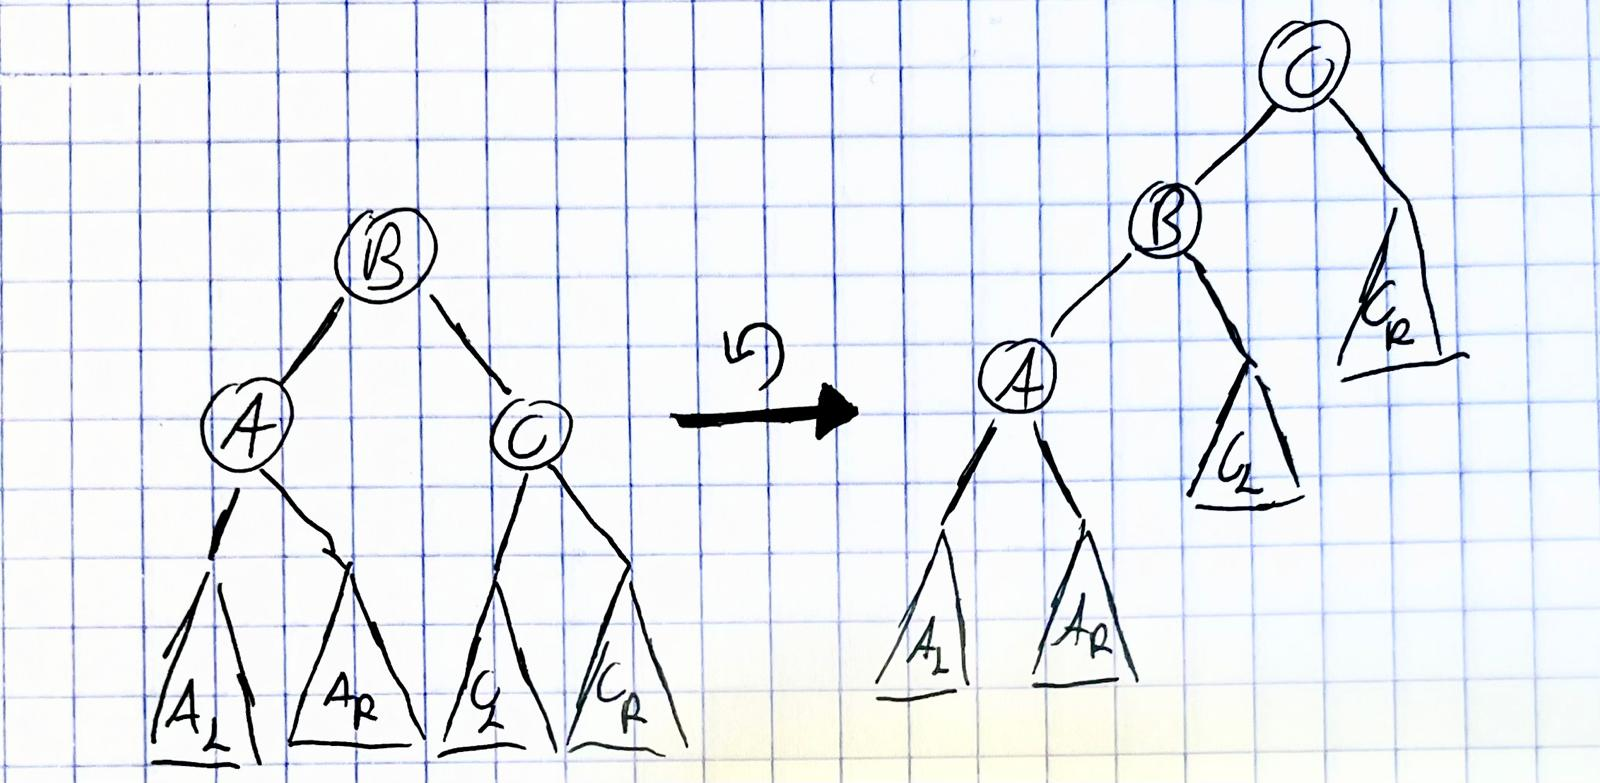
\includegraphics[width=0.35\linewidth]{images/something2}
			\end{center}
			
			ונחזור עליו (פורמלית באינדוקציה) עד שנקבל עץ מצורה של קו אחיד. משום שהגלגול הזה, במקרה הרע, יתבצע צומת עם שני עלים או (במקרה בו $A$ ריק) על צומת עם עלה שמאלי בלבד, ויש $n$ צמתים, אז כמות הגלגולים שידרשו לשם כך תהיה $O(n)$ במקרה הרע. 
			
			סה"כ ל־$T_1$ יש רצף של $O(n)$ פעולות $\ag _1 \dots \ag_k$ ע"מ להמיר אותו צורה של קו ישר עם הצומת הגבוהה ביותר למעלה, ובאופן דומה בעבור $T_2$ תהיה סדרה כזו $\bg_1 \dots \bg_n$. משום שצורה כזו יחידה, אזי $\ag_1 \dots \ag_k, \bg_n\op \dots \bg_1\op$ דרך להעביר את $T_1$ ל־$T_2$ (שכן המעבר בין $\ag_k$ לבין $\bg_k$ יתבצע על אותו העץ). זאת כאשר $\bg_i\op$ מייצג הגלגול שהופך את הגלגול $\bg_i$. סה"כ מצאנו רצף גלגולים באורך $2O(n) = O(n)$  כדרוש. 
		\end{proof}
	\end{enumerate}
	\npage
	\section{}
	נגדיר עץ $d$־ארי להיות עץ בו לכל צומת לכל היותר $d$ בנים, ונגדיר עץ $d$־ארי להיות נחמד אם לכל צומת שאינו עלה יש בדיוק $d$ בנים. 
	
	\textbf{בשאלה זו כאשר אדבר על בקיצור עץ $\bm{d}$־ארי, הכוונה לעץ $\bm{d}$־ארי נחמד. }
	\begin{enumerate}
		\item \textbf{שאלה. }מהו מספר העלים בעץ $d$־ארי נחמד בעל $n$ צמתים? \begin{proof}[תשובה. ]נתייחס לעץ כאל גרף מכוון. 
			נתבונן בעץ $d$־ארי נחמד כללי, ונסמן את מספר הצמתים \textit{שאינם} עלים ב־$k$. עתה נבין כמה עלים ישנם בעץ. ניעזר בהכלה והפרדה. $dk$ יהיה מספר הבנים שיש לכל אחד מהצמתים, וחסם עליון לכמות הצמתים בכל העץ. נבחין כי לא ספרנו שום צומת פעמים כי דרגת הכניסה של כל צומת היא $1$ לכל היותר (כלומר לא יכול להיות שצומת נספרה כבת של שני צמתים שונים). נוסיף $1$ כי לא ספרנו את השורש שאינו בן של אף צומת אחרת. 
			
			סה"כ, $n = dk + 1$. נחלץ את $d$: 
			\[ n = dk + 1 \implies n - 1 = dk \implies k = \frac{n - 1}{d} \]
			ניעזר בעקרון המשלים כדי למצוא את כמות הצמתים שהינם עלים. עולם דיון מגודל $n$ הצמתים, ו־$k$ שאינם עלים, סה"כ כמות העלים: 
			\[ n - k = n - \frac{n - 1}{d} = \bm{\frac{n(d - 1) + 1}{d}} = \ans \]
			\textit{הערה: }נבחין כי התשובה לא מוגדרת אמ"מ $d$ לא מחלק את $n - 1$, שכן אז ישנה כמות לא שלמה של עלים. במקרה כזה נסיק שלא קיים עץ $d$־ארי נחמד מתאים ל־$n$ צמתים, מצב שייתכן. 
		\end{proof}
		\item \textbf{שאלה. }בהינתן עץ $d$־ארי נחמד בגובה $h$ עם $L$ עלים, הוכיחו שמתקיים $L \le d^h$.
		\begin{proof}[תשובה.]ננסה למצוא את העץ המקסימלי האפשרי בהינתן גובה $h$. נבחין כי אם העץ לא מאוזן, אזי ישנו צומת שבמרחק $h - i, \ i > 0$ מהשורש, כלומר נוכל להוסיף לו צומת נוסף ולשמור על גובה $h$, ועל כן הוא אינו מקסימלי (מבחינת כמות הצמתים). לכן העץ המקסימלי מאוזן. 
			\begin{center}
				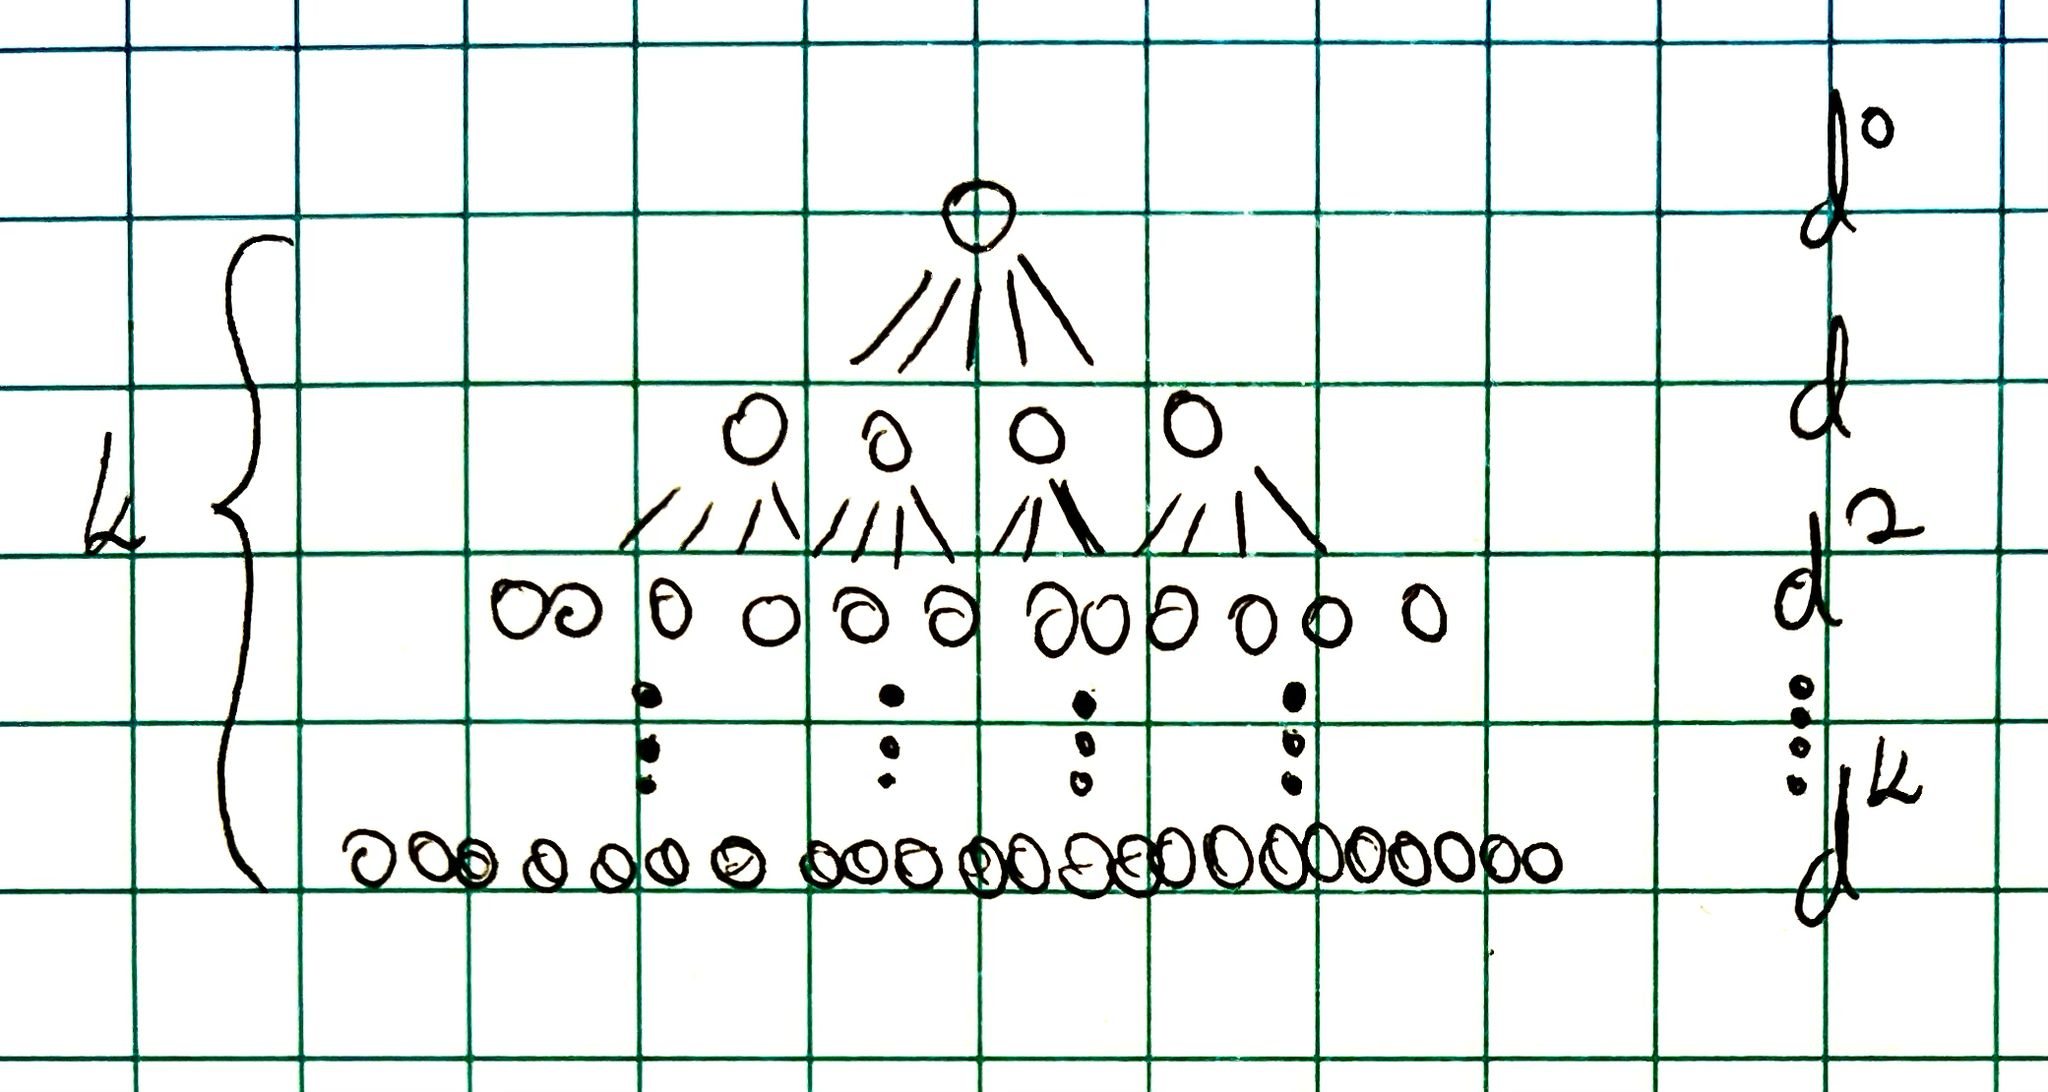
\includegraphics[width=0.35\linewidth]{images/something}
			\end{center}
			נבחין שבשכבה ה־$i$ ישנם $d^{i - 1}$ צמתים (פורמלית, יש $d^{i - 1}$ במרחק $i$ מהשורש) [הוכחה לטענה הזו בסוף ההוכחה]. לכן כמות הצמתים הכוללת היא: 
			\[ n = \sum_{i = 1}^{h}d^{i - 1} = \sum_{i = 0}^{h - 1}d^{i} = \frac{d^{h} - 1}{d - 1} \]
			ולכן, מסעיף (א), כמות העלים בעץ כזה: 
			\[ L = \frac{\frac{d^{h} - 1}{d - 1}(d - 1) + 1}{d} = \frac{d^{h} \cancel{ - 1 + 1}}{d} = d^{h - 1} \]
			שכאמור מהווה חסם עליון לכמות הצמתים בכל עץ $d$־ארי נחמד, וסה"כ החסם העליון לכמות הצמתים הוא $L \le d^{h - 1} \le d^h$ כדרוש. 
			
			[הוכחה לכך שכמות הצמתים במרחק $i$ מהשורש היא $d^{i - 1}$: בסיס עץ עם צומת אחד, שכבה אחת ו־$d^{1 - 1} = d^0 = 1$ צמתים כדרוש, צעד נניח באינדוקציה על $i$ ונוכיח על $i + 1$, אזי לכל אחד מ־$i$ הצמתים יש $d$ בנים הם היחידים ממרחק $i + 1$ (קשת נוספת בינהם לבין אביהם במרחק $i$), ומה.א. יש $d^{i - 1}$ צמתים במרחק $i$ ולכן סה"כ ישנם $d \cdot d^{i - 1} = d^{(i + 1) - 1}$ צמתים במרחק $i + 1$ כדרוש]
		\end{proof}
			
	\end{enumerate}
	
%	\begin{enumerate}
%		\item \textbf{שאלה. }בהינתן $n$ צמתים, מהו מספר העלים בעץ $d$־ארי נחמד? \begin{proof}[פתרון. ]
%			ראשית, ננסה להבין אילו ערכי $n$ תקינים להיות כמות הצמתים בעץ $d$־ארי. נסמן את עומק עץ כלשהו ב־$k$, ונבחין כי בכל "שכבה" (קבוצת צמתים ממרחק $i$ מהשורש) יש $d^i$ צמתים (ראה איור). 
%		\end{proof}
%		\begin{center}
%			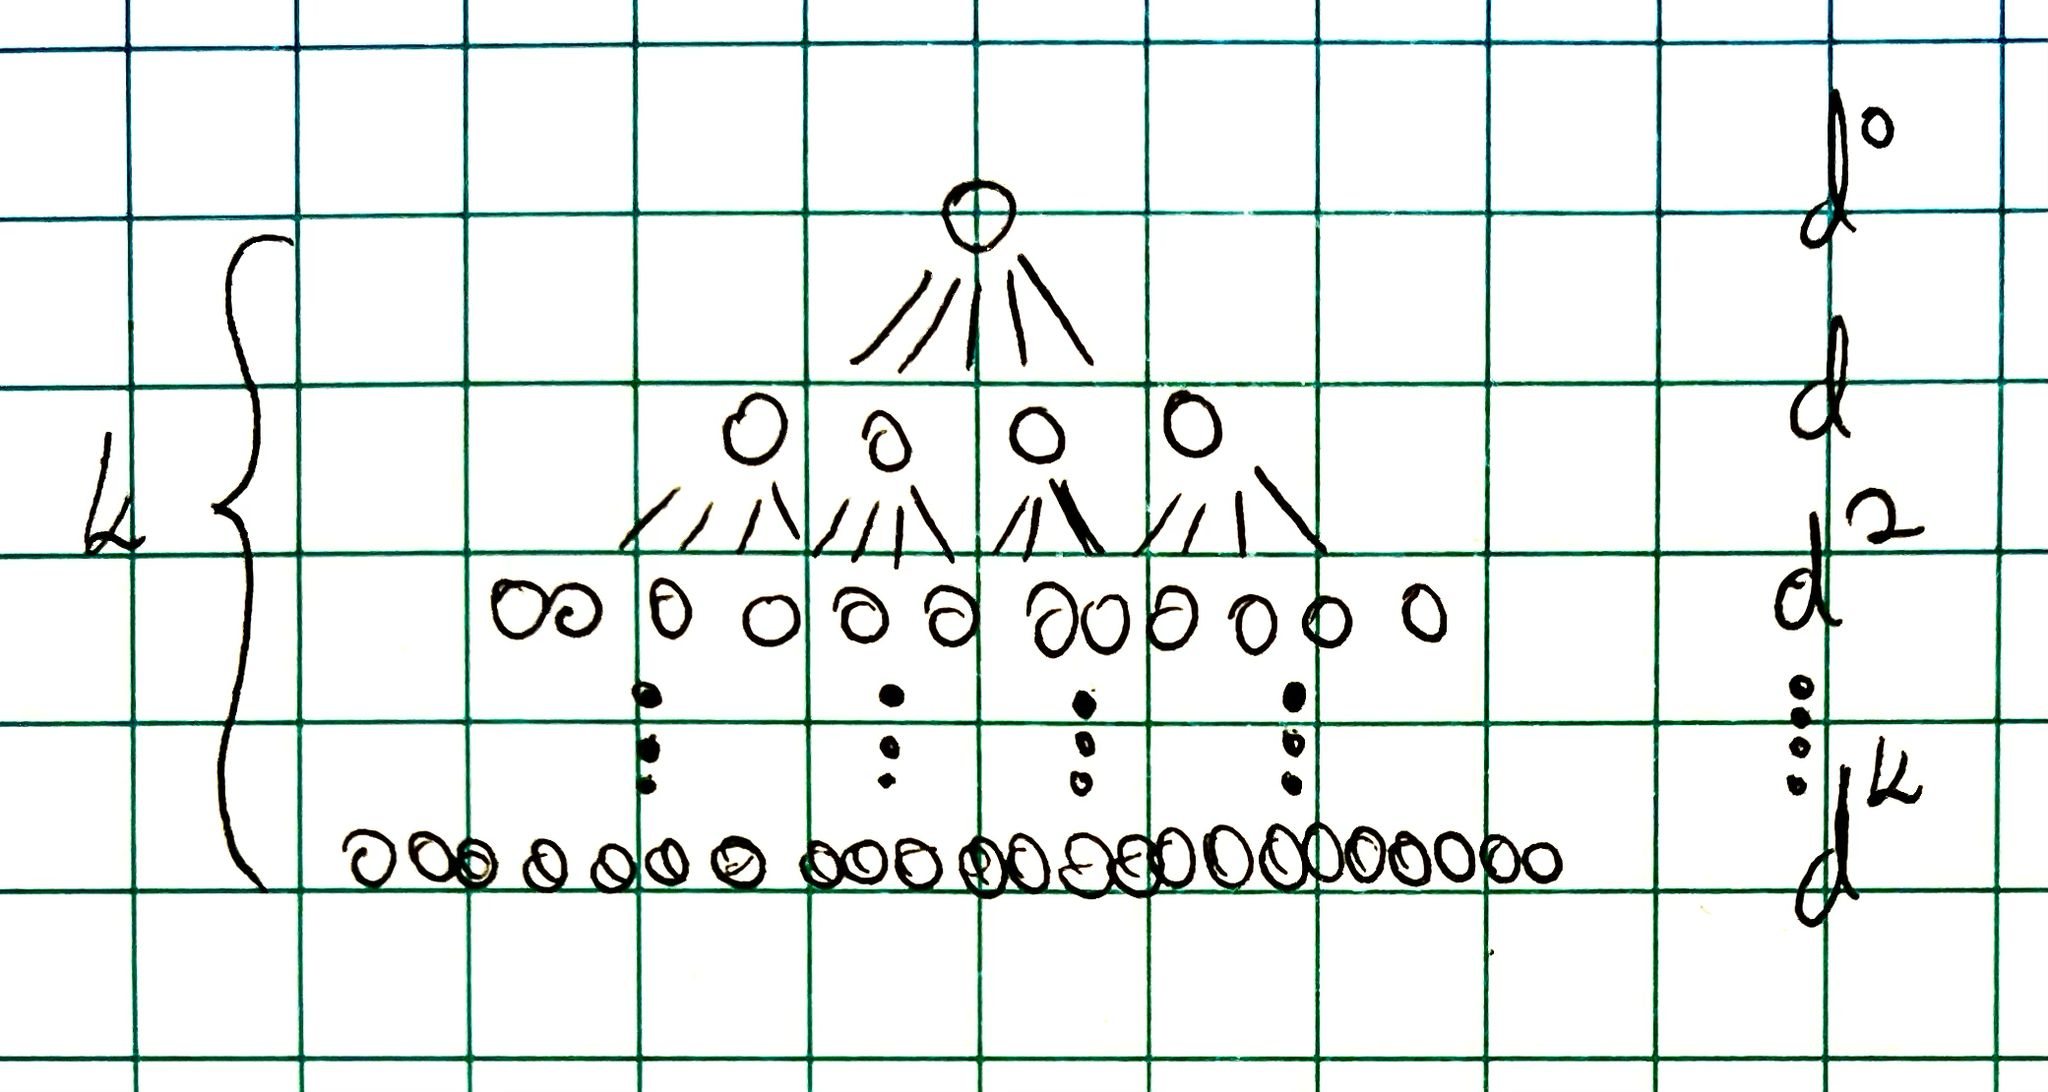
\includegraphics[width=0.35\linewidth]{images/something}
%		\end{center}
%		לכן, כמות הצמתים בעץ מעומק $i$ היא $n = \sum_{i = 1}^{k}d^i = \frac{d^k - 1}{d - 1}$. במילים אחרות, קיים $k$ כך ש־$n = \frac{d^k - 1}{d - 1}$ כך ש־$n$ מספר הצמתים של עץ $d$־ארי נחמד כלשהו. עוד נבחין מהאיור שכמות העלים בעץ היא $d^k$. ניעזר במשוואה: 
%		\[ n = \frac{d^k - 1}{d - 1} \implies n(d - 1) = d^k - 1 \implies d^k = nd - n - 1 \]
%		במילים אחרות, כמות העלים היא $nd - n - 1$. 
%		\item בהינתן עץ $d$־ארי נחמד בגובה $h$ עם $L$ עלים, צ.ל. $L \le d^h$. \begin{proof}
%			נבחין בשינויים מהסימונים של הסעיף הקודם – $h := k, \ L := n$. משום שיש בעץ $d^h$ עלים (ראה סעיף קודם) אז מתקיים $L = d^h \le d^h$ כדרוש. 
%		\end{proof}
%	\end{enumerate}
	
	\npage
	\section{}
	\begin{multicols}{2}
		\subsection*{סעיף א'}
		להלן פסאדו קוד (רקורסיבי) שבודק האם עץ בינארי הוא עץ חיפוש: 
		{\sen\begin{algorithm}[H]
				\DontPrintSemicolon
				\importDs\sFunc{RecSearch}\sData{T}\sData{node}\sData{left}\sData{right}\sData{isSearch}\sData{rightVal}\sData{leftVal}\sData{recCall}\sFunc{min}\sFunc{max}\sData{leftMax}\sData{rightMin}
				\io{Binary tree \T}{Whether is \T a search tree}
				\Fn{\RecSearch{\node} $\to$ {boolean, max, min}}{
					\If{$\node = \Null$}{
						\KwRet{{\True, $-\inf$, $+\inf$}}
					}
					\left $\gets$ \node.left\;
					\right $\gets$ \node.right\;
					\leftMax $\gets$ $-\inf$\;
					\rightMin $\gets$ $+\inf$\;
					\isSearch $\gets$ \True\;
					\uIf{$\right \neq \Null$}{
						\recCall $\gets$ \RecSearch{\right}\;
						\leftMax $\gets$ \recCall\!\![1]\;
						\isSearch $\gets$ \recCall\!\![0] \bf and \isSearch \bf and \textbackslash\textbackslash\; \quad\quad \node.item $>$ \leftMax\;
					}\ElseIf{$\left \neq \Null$}{
						\recCall $\gets$ \RecSearch{\left}\;
						\rightMin $\gets$ \recCall\!\![2]\;
						\isSearch $\gets$ \recCall\!\![0] \bf and \isSearch \bf and \textbackslash\textbackslash\; \quad\quad \node.item $<$ \rightMin\;
					}
					\KwRet{\isSearch, \max{\node.item, \leftMax}, \bf\textbackslash\textbackslash\; \quad\quad \min{\node.item, \rightMin}}
				}
				
				\KwRet{\RecSearch{\T.root, $-\inf$, $+\inf$}}\;
			\end{algorithm}\she}
		(הערה: \textbackslash\textbackslash \, מציין מעבר שורה מפאת מקום מבלי לקטוע את ההצרה)
		
		נוכיח שהסיבוכיות היא $O(n)$. נניח בשלילה שתקרא קריאה רקורסיבית פעמיים לאותו האיבר, אז משום שקריאות רקורסיבית מתבצעות אך ורק לצמתים המחוברים בצומת אחת לצומת האב, אזי אפשר להרכיב מעגל (לא מכוון) מן הצומת לעצמה, למרות שבעץ אין מעגלים כאלו וסתירה. יש $n$ אפשרויות שונות לקלטי הפונקציה, הם צמתי העץ, הראינו כי לא נחזור על אותו הצומת פעמיים, וסה"כ יהיו לכל היותר $n$ קריאות רקורסיביות. משום שבפנים כל הפעולות פעולות השוואה ושמירת מידע בזכרון (עד לכדי פעולות רקורסיביות שכבר ניתחנו), סה"כ הסיבוכיות היא $O(n)$. 
		\vfill\null
		\columnbreak
		\subsection*{סעיף ב'}
		הגיון: נשמור ב־\texttt{mode} את המצב הנוכחי (קורא שמאלה או קורא ימינה) וב־\texttt{heads} את הצמתים שעליהם עברנו ומצטרך לחזור אילהם. המצבים הם $0$ כאשר זז שמאלה, $1$ כאשר ימינה, ו־$2$ כאשר סיימנו לזוז ימינה ויש צורך לעבור לצומת האב הבא. 
		{\sen\begin{algorithm}[H]
				\DontPrintSemicolon
				\importDs\sData{T}\sData{heads}\sData{mode}\sData{left}\sFunc{Print}\sData{right}
				\io{\T binary tree}{nothing}
				\heads $\gets$ \Stack{} \tcp*[r]{Top, Pop \& Push in $O(1)$}
				\mode $\gets$ 0\;
				\Push{\heads, \T.root}\;
				\While{$\Top{\heads} \neq 0$}{
					\tcp*[f]{\mode $=$ 0}\\[-\baselineskip]
					\uIf{$\mode = 0$}{
						\left $\gets$ \Top{\heads}.left\;
						\eIf{$\left \neq \Null$}{
							\Push{\heads, \left} \;
						}{
							\Print{\Top{\heads}}\;
							\mode $\gets$ 1\;
						}
						\tcp*[f]{\mode $=$ 1}\\[-\baselineskip]
					}\uElseIf{$\mode = 1$}{
						\right $\gets$ \Top{\heads}.right\;
						\eIf{$\right \neq \Null$}{
							\Push{\heads, \right}\;
							\mode $\gets$ 0\;
						}{
							\Pop{\heads}\;
							\mode $\gets$ 2
						}
						\tcp*[f]{\mode $=$ 2}\\[-\baselineskip]
					}\ElseIf{$\mode = 2$}{
						\Pop{\heads}\;
						\mode $\gets$ 1
					}
				}
			\end{algorithm}\she}
		
		הסיבוכיות של האלגוריתם לינארית כי הוא מבצע ישירות מעבר על הצמתים in-order, בלי לעבור על שום צומת פעמיים. 
	\end{multicols}
	
	\ndoc
\end{document}